\cotefile{72}
\scanpage{51}
% top, lines 1–2
\[
\left\{\begin{aligned}
\delta_n(B_0,\ldots,B_{n-1})&=B_0^n B_1^{n-1}\cdots B_{n-1}L_n(B_1,\ldots,B_{n-1})\\
\delta_{n+1}(1,B_0,\ldots,B_{n-1})&=B_0^n B_1^{n-1}\cdots B_{n-1}L_{n+1}(B_0,B_1,\ldots,B_{n-1})
\end{aligned}\right.
\]

% upper, lines 3–4
\[
\left\{\begin{aligned}
\unsure{F|\delta}'_n\deleted{\unsure{=}}(B_0,\ldots,B_{n-1})&=B_0^n\deleted{B_1}^{n-1}B_{n-1}L'_n(B_1,\ldots,B_{n-1})\\
\delta'_{n+1}(1,B_0,\ldots,B_{n-1})&=B_0^n B_1^{n-1}\cdots B_{n-1}L'_{n+1}(B_0,B_1,\ldots,B_{n-1})
\end{aligned}\right.
\]

% upper middle, line 5
\deleted{\unsure{On va faire|$n$ pair}}

% upper middle, lines 5–6
\[
\left\{\begin{aligned}
&\deleted{L_n(B_1,\ldots,B_{n-1})\equiv B_1 B_3\cdots B_{n-1}}\\
&\deleted{\delta_n(}
\end{aligned}\right.
\]

% right of cancelled display
\figure{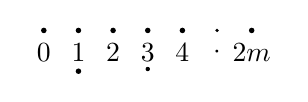
\begin{tikzpicture}[x=.44cm,y=.28cm]
\foreach \x/\a in {0/0,1/1,2/2,3/3,4/4,6/2m}{\fill (\x,1) circle (1pt);\node at (\x,0) {$\a$};}
\fill (5,1) circle (.65pt);\node at (5,0) {$\cdot$};
\fill (1,-.85) circle (1pt);\fill (3,-.75) circle (.8pt);
\end{tikzpicture}}

% middle, lines 7–9
\[
\begin{aligned}
L_{2m}(B_1,\ldots,B_{2m-1})&\equiv B_1B_3\cdots B_{2m-1}\qquad \text{\uuline{mod 2}}\\
L'_{2m+1}(B_1,\ldots,B_{2m})&\equiv (B_2 B_4\cdots B_{2m}+B_1 B_3\deleted{\unsure{B_5 B_{\unsure{7}}}}\cdots B_{2m-1})\\
&\quad+\sum_{1\le i\le m-1}(B_1\cdots B_{2i-1})(B_{2i+2}\cdots B_{2m})
\end{aligned}
\]

% lower middle, lines 10–13
\[
\left\{\begin{aligned}
\delta_{2m}^{\unsure{\prime}}(B_0,\ldots,B_{2m-1})&\equiv
\deleted{(B_0^{2m}B_1^{2m-1}\cdots B_{2m-1}}
\underbrace{(B_0 B_1)^{2m}(B_2B_3)^{\unsure{2(m-1)|2m-1}}\cdots(B_{2m-2}B_{2m-1})}_{\displaystyle [(B_0B_1)^m(B_2B_3)^{m-1}\cdots(B_{2m-2}B_{2m-1}]^2}\\
\delta'_{2m+1}(1,B_0,\ldots,B_{2m-1})&\equiv B_0^{2m} B_1^{2m-1}\cdots B_{2m-1}\bigl[B_0B_2\cdots B_{2m-2}+B_1B_3\cdots B_{2m-1}\\
&\qquad+\sum_{1\le i\le m-1}(B_0\cdots B_{2i-2})(B_{2i+1}\cdots B_{2m-1})\unsure{]}
\end{aligned}\right.
\]

% lower, lines 14–16
\[
\left\{\begin{aligned}
\delta'_{2m+1}(B_0,\ldots,B_{2m})&\equiv B_0^{2m+1}B_1^{2m}\cdots B_{2m}\bigl(\deleted{\unsure{B_0}}B_2 B_4\cdots B_{2m}+ B_1B_3\cdots B_{2m-1}\\
&\qquad+\sum_{1\le i\le m-1}(B_1\cdots B_{2i-1})(B_{2i+1}\cdots B_{2m})\bigr)\\
\delta_{2m+2}(1,B_0,\ldots,B_{2m})&\equiv\deleted{(B_0^{\unsure{2m+1}}B_1^{\unsure{m+1}}\unsure{\cdots})}
\bigl[B_0^{m+1}(B_1 B_2)^m\unsure{\cdots}(B_{2m-1}B_{2m})\bigr]^2
\end{aligned}\right.
\]

% foot, left
% archive sheet number: 50

\scanpage{52}
% top, line 1
\[
\Delta_n(\deleted{\unsure{C_0}}B_0,\ldots,\unsure{C_n|B_n|C_{n-1}})
=2\unsure{B_0|C_0}\Delta_{n-1}(\unsure{C_1|B_1},\ldots,C_{n-1})-C_1^2\Delta_{n-2}(\unsure{B_2|C_2},\ldots,C_{n-1})
\]

% upper, lines 2–5
\[
\shortparallel
\]
\[
\begin{aligned}
\delta_n(B_0,\ldots,B_{n-1})&=2B_0\delta_{n-1}(B_0B_1,B_2,\ldots,B_{n-1})-(B_0B_1)^2\delta_{n-2}(B_0B_1B_2,B_3,\ldots,B_{n-1})\\
\text{''}\quad &=2B_0^{\unsure{1}}(B_0B_1)^{n-1}B_2^{n-2}B_3^{n-3}\cdots B_{n-1}L_{n-1}(\deleted{B_0}B_2,B_3,\ldots,B_{n-1})\\
B_0^n\cdots B_{n-1}L_n(B_1,\ldots,B_{n-1})&\qquad-B_0^2B_1^2(B_0 B_1 B_2)^{n-2}B_3^{n-3}\cdots B_{n-1}L_{n-2}(B_3,\ldots,B_{n-1})\\
&=B_0^n B_1^{n-1}\cdots B_{n-1}\bigl[2L_{n-1}(B_2,\ldots,B_{n-1})-B_1L_{n-2}(B_3,\ldots,B_{n-1})\bigr]
\end{aligned}
\]

% upper, line 6, boxed
\[
\boxed{L_n(B_1,\ldots,B_{n-1})=2L_{n-1}(B_2,\ldots,B_{n-1})-B_1 L_{n-2}(B_3,\ldots,B_{n-1})}
\]

% middle, lines 7–8
\[
\left\{\begin{aligned}
L_{2m}^{\deleted{\unsure{\prime}}}(B_1,\ldots,B_{2m-1})&=4L'_{2m-1}(B_2,\ldots,B_{2m-1})-B_1L_{2m-2}(B_3,\ldots,B_{2m-1})\\
L'_{2m+1}(B_1,\ldots,B_{2m})&=\deleted{2}L_{2m}(B_2,\ldots,B_{2m})-B_1L'_{2m-1}(B_3,\ldots,B_{2m})
\end{aligned}\right.
\]

% middle, line 9
Calcul du $\unsure{\widetilde{o}|\widetilde{\sigma}|\widetilde{c}}$ défini par

% middle, lines 9–10
\[
\begin{aligned}
&\overset{\shortparallel}{\zeta_{-1}a_{-1}}+\zeta_0a_0\cdots+\zeta_n a_n
&\left\{\begin{aligned}\zeta_n&=1\\ \langle\widetilde{o},a_{0}^{\prime}\rangle&=0\qquad 0\le i\le n\end{aligned}\right.
\end{aligned}
\]

% middle, line 11, left
i.e.

% lower middle, lines 11–14
\[
\left\{\begin{aligned}
\zeta_n&=1\\
\zeta_{n-1}&=2\\
\{\ \zeta_{i-1}-2\zeta_i+\beta_i\zeta_{i+1}&=0\qquad 0\le i\le n-1\\
\zeta_{i-1}&=2\zeta_i-\beta_i(\zeta_{i+1})
\end{aligned}\right.
\]

% lower, line 15
\[
\begin{aligned}
\zeta_n=1,\quad \zeta_{n-1}=2,\quad \zeta_{n-2}&=\deleted{\unsure{2}}4-\beta_{n-1},\\
\zeta_{n-3}&=2(4-\beta_{n-1})-2\beta_{n-2}\cdot\deleted{\unsure{2}}\unsure{1}=8-2(\beta_{n-1}+\beta_{n-2}\unsure{)}
\end{aligned}
\]

% lower, line 16, boxed
\[
\boxed{\zeta_{n-i}=L_i(\underbrace{\beta_{n-1},\ldots,\beta_{n-i+1}}_{i-1\ \text{arguments}})}
\qquad 1\le i\le n+1
\]

% right, below box
en particulier

% foot, lines 17–18
\[
\begin{aligned}
\rho&=\bar{\zeta}_{-1}=\pi(\widetilde{o})=L_{n+1}(\beta_{n-1},\ldots,\beta_0)=L_{n+1}(\beta_0,\ldots,\beta_{n-1})\\
\sigma&=\zeta_0=\langle\widetilde{o},a_0^*\rangle\bigl[=-\langle\widetilde{o},\psi(\underset{\shortparallel\,s_0}{a_{-1}})\rangle
=-\varphi(\widetilde{o},a_{-1})\deleted{\unsure{=\langle a_{-1},\psi(a)\rangle}}\inserted{=-\langle a_{-1},\psi(\widetilde{o})\rangle}\bigr]
\equiv \begin{aligned}&L_n(\beta_{n-1},\ldots,\beta_1)\\[-2pt]&\text{''}\,L_n(\beta_1,\ldots,\beta_{n-1})\end{aligned}
\end{aligned}
\]

% foot, left
% archive sheet number: 51

\scanpage{53}
% top, lines 1–2
\[
\begin{aligned}
\rho&=L_{n+1}(\beta_0,\ldots,\beta_{n-1})&\rho'&=L'_{n+1}(\beta_0,\ldots,\beta_{n-1})\\
\sigma&=L_n(\beta_{\unsure{1|0}},\ldots,\beta_{n-1})&\sigma'&=L'_n(\beta_1,\ldots,\beta_{n-1})
\end{aligned}
\]

% upper, lines 3–4
\[
\left\{\begin{aligned}\delta_{\unsure{E|\mathcal E|\varepsilon|\Sigma}}&=(\overbrace{\beta_0^n\beta_1^{n-1}\cdots\beta_{n-1}}^B)\sigma\\
\delta_V&=(\underbrace{\beta_0^n\beta_1^{n-1}\cdots\beta_{n-1}}_B)\rho\end{aligned}\right.
\quad
\left\{\begin{aligned}\delta'_E&=(\overbrace{\beta_0^n\beta_1^{n-1}\cdots\beta_{n-1}}^B)\sigma'\\
\delta'_V&=(\underbrace{\beta_0^n\beta_1^{n-1}\cdots\beta_{n-1}}_B)\rho'\end{aligned}\right.
\]

% upper right, lines 4–5
\margin{$\unsure{\widetilde{o}|\widetilde{\sigma}|\widetilde{c}}=\rho a_{-1}+\sigma a_0+\zeta_1a_1\cdots+\zeta_na_n$\quad $(\zeta_n=1,\zeta_{n-1}=2\ldots)$}

% upper middle, lines 5–6
\[
\begin{aligned}
\rho&=\zeta_{-1}=\pi(\widetilde{o})=\langle\widetilde{o},a_{-1}^*\rangle\\
\sigma&=\zeta_0=\langle\widetilde{o},a_0^*\rangle=-\varphi\underbrace{(s_i,\widetilde{o})}_{0\le i\le n}
\end{aligned}
\qquad
\left\{\begin{aligned}
o&=\widetilde{o}/\rho\quad o'=2o=\deleted{\unsure{\widetilde{o}/\rho}}\begin{cases}\deleted{\unsure{2}}\widetilde{o}/\rho'&n\ \text{pair}\\2\widetilde{o}/\rho&n\ \text{impair}\\ \text{''}\ 2\bar{o}/\rho'&\end{cases}\\
\psi(\widetilde{o})&=-\sigma a_{-1}^*=-\sigma\pi
\end{aligned}\right.
\]

% middle, lines 7–8
\[
\begin{aligned}
f(\widetilde{o})&=\bigl[\tfrac12\langle\widetilde{O},\psi(\widetilde{o})\rangle=-\tfrac12\langle\widetilde{o},\sigma\pi\rangle=-\tfrac12\sigma\pi(\widetilde{o})=-\tfrac12\sigma\rho\bigr]=-\deleted{\unsure{\sigma}}\sigma'\rho'\\
\bigl[f(o')&\underset{\text{\unsure{(n pair|en pair}}}{=} f(\widetilde{o}/\rho')=\deleted{\unsure{\tfrac12}}-\frac{\sigma'\rho'}{\rho'^2}\deleted{\unsure{\tfrac12}}=-\frac{\sigma'}{\rho'}\bigr]
\end{aligned}
\]

% middle, lines 9–10
\[
\begin{aligned}
f_E\ \text{lisse}&\Longleftrightarrow\text{ les }\beta_i\ (0\le i\le n-1)\ \text{inversibles, et }\sigma'\ \text{inv.}\\
&\underset{\substack{\text{si }2\ \text{inv.}\\\text{ou }n\ \text{pair}}}{\Longleftrightarrow}\text{ les }\beta_i\ \text{inv. et }\psi(\widetilde{o})\ne0
\end{aligned}
\]

% lower middle, lines 11–12
\[
\begin{aligned}
f_V\ \text{lisse}&\Longleftrightarrow\text{ les }\beta_i\ (0\le i\le n-1)\ \text{inversibles, et }\rho'\ \text{inv.}\\
&\underset{\substack{\text{si }2\ \text{inv.}\\\text{ou }n\ \text{impair}}}{\Longleftrightarrow}
\text{ les }\beta_i\ \text{inv. et }\underbrace{\pi(\widetilde{o})\ne\text{\unsure{zéro|inv.}.}}_{\substack{\text{centre, à dist.}\\\text{finie sur tte fibre}}}
\end{aligned}
\]

% lower, line 13
\[
(E,V,f)\ \text{\unsure{birégulier}}\Longleftrightarrow
\text{ les }\beta_i\ (0\le i\le n-1)\ \text{inv. \uline{et} }f(\widetilde{o})\ \text{\uline{inv.}}
\]

% near foot, cancelled block
\deleted{\uline{NB} \uline{si $n$ pair}, $\pi(o')=\pi(\widetilde{o}/\rho')=\rho/\rho'=2$}

% foot, left
% archive sheet number: 52

\scanpage{54}
% heading
Antipodisme

% top, lines 2–4
\[
\begin{aligned}
&\deleted{x\longmapsto 2\unsure{o|c}\,\pi(x)-x}\\
\underline a&=-\mathrm{id}+\deleted{\unsure{2\pi\otimes o}}2\pi\otimes o=-\mathrm{id}+\pi\otimes o'\\
-\underline a&=\mathrm{id}-\pi\otimes o'
\end{aligned}
\]

% upper right
\margin{\uline{Attention} il se peut que \unsure{$c''$|$c'$} n'existe pas ``à dist. finie'', mais c' existe\ldots}

% upper, lines 5–7
\uline{NB} $\underline a$ défini sss $c'$ défini i.e. sss $\rho'$ inversible (c'est le cas si $f_V$ lisse). Notons que $\overbrace{\rho' o'=\unsure{\widetilde{o}|\widetilde{\sigma}|\widetilde{c}}}^{\text{si }n\ \unsure{impair|pair}}$ partt $\ne0$ donc $o'$ partt $\ne0$ donc $\mathcal O_S o'=\mathcal O_S\widetilde{o}$.

% slanted, upper left
% slanted
\margin{\uline{NB} Si $n$ pair ou $2$ inv, alors : $\underline a$ défini \uline{et} est une réflexion \uuline{str.} \uline{orth.} $\Longleftrightarrow\sigma'\rho'$ inv, i.e. $\sigma'$ et $\rho'$ inv.}

% upper middle, lines 7–10
$\langle o',\pi\rangle=2$, donc $-\underline a$ est une réflexion, sauf si en certains pts on a car. $=2$, \uline{et} \deleted{\unsure{alors}} \deleted{ce qui} rang impair
\margin{$\bar m$ \unsure{conclusion|conditions} pour \unsure{les|tts} points où 2 inv. Mais en car 2 pour $n$ imp. on a $o'=0$ d'où $\underline a=\mathrm{id}$.}

% upper middle, line 11
$\underline a$ commute aux $\tau_i$, il inverse $o$, $c'$ etc.

% upper middle, line 12
\[
\underline a(s_0)=\underline a(a_{-1})=\deleted{\unsure{2o-s_0}}o'-s_0=\widetilde{s}_0
\]

% middle, lines 13–15
\uline{NB} Dans $\unsure{E|\mathcal E}$, l'ens. des pts fixes de $\underline a$ est \deleted{\unsure{$\mathcal O_S o=\mathcal O_S$}} la droite engendrée par $o'$ si $2$ inv -- si $2\,1_S=0$ i.e. $S$ de car. 2, alors \deleted{\unsure{o'|c'est l'}} ens des pts fixes est $V$.

% middle, lines 16–18
Dans $\mathrm P(E)$, l'ens des pts fixes est $\mathrm P(V)\cup\{o'\}$ -- qui se réduit à $\mathrm P(V)$ en car. 2

On a $s_0\ne\widetilde{s}_0=\underline a\,s_0$ dans $\mathrm P(E)=X$.

% middle lower, line 19
Considérons le \deleted{droite} plan engendré par $s_0$ et $\widetilde{o}$ \deleted{\unsure{(ou $o'$)}}

% lower, line 20
\[
g(\lambda,\mu)=f(\lambda s_0+\mu\widetilde{o})=\deleted{\unsure{\tfrac12 f\lambda}}\lambda\mu\underbrace{\varphi(s_0,\widetilde{o})}_{-\zeta_0=-\sigma}+\mu^2 f(\widetilde{o})=-\sigma\lambda\mu-\sigma'\rho'\mu^2=-\mu(\sigma\lambda+\sigma'\rho'\mu)
\]

% lower, line 21
1) \uline{$n$ pair} : $\sigma=\sigma'$, $\rho=2\rho'$\qquad $f(\lambda s_0+\mu\widetilde{o})=-\mu\sigma(\lambda+\rho'\mu)$

% lower left, lines 22–29
\margin{\uline{NB} Si $\sigma$ inv. \deleted{\unsure{pour}} \inserted{pour} $f(\lambda s_0+\mu\widetilde{o})=0$, $\mu$ inv. sss $\lambda+\rho'\mu=0$ i.e. $\lambda=-\rho'\mu$ i.e. $(\lambda,\mu)\mathrel{\#}(-\rho',1)$ donc $\lambda s_0+\mu\widetilde{o}$ multiple de $-\rho's_0+\widetilde{o}$ ou encore (si $\rho'$ inv) de $-s_0+\frac{\widetilde{o}}{\rho'}=-s_0+o'=\widetilde{s}_0$}

% lower right, lines 22–30
\[
\begin{aligned}
&\text{c'est }=0\text{ sss }\sigma=0\\
&\text{c'est }\ne0\text{ en chaque fibre }\overset{\unsure{\text{sss}|\text{ssi}}}{\Longleftrightarrow}\sigma\ \text{inv. i.e. }\sigma'\ \text{inv.}\\
&\deleted{\text{dans ce cas,}}\inserted{\Longleftrightarrow}\quad Q_X\cap D_0\ \text{est un rev. étale de}\\
&\text{degré 2 de }S,\text{ dont }s_0\text{ est une section,}\\
&[\underline a_X s_0\text{ est la section complémentaire,}\\
&\hspace{3em}\text{quand }\underline a_X\text{ est définie}]\\
&\Longleftrightarrow Q_X\not\supset D_0\ \text{en tte fibre}\\
&\hspace{3em}(\text{c'est le cas si }f_E\ \text{lisse})\\
&\Longleftrightarrow\psi(\widetilde{o})\ne0\ \text{chaque fibre}\Longleftrightarrow(\widetilde{o})^\perp=V\ \text{chaque fibre}
\end{aligned}
\]

% foot, line 31
2) \uline{$n$ impair}\qquad $\sigma=2\sigma',\ \rho=\rho',$\qquad $f(\lambda s_0+\mu\widetilde{o})=-\mu\sigma'(2\lambda+\rho'\mu)$

% foot, left
% archive sheet number: 53

\scanpage{55}
% top, lines 1–4
A) \uline{2 inv.}\quad \deleted{Alors $f(\lambda s_0+\mu\unsure{\widetilde{o}|\widetilde{\sigma}|\widetilde{c}})=0$ $\forall\lambda,\mu$ \inserted{$g(\lambda,\mu)$ est ident} sss \unsure{$\sigma'$|$\sigma$}} Alors, indépendamment de la parité de $n$, on peut écrire $g(\lambda,\mu)=-\sigma\mu(\lambda+\frac{\rho}{2}\mu)$, et les équivalences décrites dans 1°) sont valables, avec $\rho'$ remplacé par $\rho/2$.

% upper left, line 5
\deleted{b) $S$ de car. 2}

% upper, lines 5–8
Les solutions de $g(\lambda,\mu)=0$, avec $\mu$ inv, sont multiples de $(-\frac{\rho}{2},1)$ et correspondent à $-\frac{\rho}{2}s_0+\widetilde{o}$ ou encore \deleted{$-\unsure{\rho/2}s_0+o$} (si $\rho$ inv. i.e. $\underline a$ défini)
\[
-s_0+2\frac{\widetilde{o}^{\unsure{+}}}{\rho}=o'-\beta_0=\underline a\,s_0
\]

% upper middle, lines 9–10
B) $2\cdot1_S=0$ i.e. $S$ de car. 2. On trouve alors \deleted{$f(\lambda s_0+\mu\widetilde{o})$}

% upper middle, lines 10–12
\[
\begin{aligned}
g(\lambda,\mu)&=f(\lambda s_0+\mu\widetilde{o})=\unsure{+|-|\deleted{-}}(\sigma'\rho')\mu^2\\
&\text{c'est }\equiv0\text{ sss }\sigma'\rho'=0\\
&\text{c'est }\ne0\text{ en tte fibre sss }\sigma'\rho'\text{ inv. i.e. }\sigma'\text{ et }\text{\uuline{$\rho'$}}\text{ inv.}
\end{aligned}
\]

% middle left
\margin{$\underline a\,x=x+o'=x$ \deleted{$f(x+o')=f(x)+f(o')+\langle x,\psi(o')\rangle$} car comme $\rho=\rho'$, \unsure{$s$}}

% middle, lines 13–16
i.e. $\sigma'$ inv et $\underline a$ \deleted{\unsure{$E$|$\mathcal E$}} défini (c'est le cas si $(E,V,f)$ birégulier). \deleted{\unsure{Il}} Ceci signifie aussi $D_0\not\subset Q_X$ en ttes fibres, et implique que $D_0$ est tangente à $Q_X$

% middle, horizontal rules
\figure{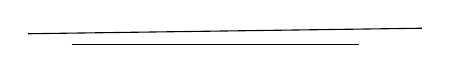
\begin{tikzpicture}\draw (0,0)--(5,.07);\draw (.55,-.14)--(4.2,-.14);\end{tikzpicture}}

% lower, lines 17–25, crossed by two long strokes
\deleted{Supposons $n$ pair, $n=2m$. On s'intéresse aux systèmes $(X,\tau_*=(\tau_i)_{0\le i\le n},s_0)$ \deleted{\unsure{tels}} non dégénérés, et tels que $\sigma\ (= \sigma')$ soit inv. [Si on suppose déjà les $\beta_i$ (i.e. $0\le i\le n-1$) inv, celà signifie $f_E$ lisse.] \deleted{Ceci définit donc} Ceci définit donc $(X,\underset{\text{\unsure{hyperquadrique|hyp. quadrique}}}{Q_X},\tau_*^X)$, où maintenant les $\tau_*$ \inserted{$(0\le i\le n)$} sont des autom. \deleted{de} involutifs de $(X,Q_X)$. Considérons la restriction :}

% lower, last line
\[
(C,Q_C,\tau_*^C)\quad -
\]

% foot, left
% archive sheet number: 54

\scanpage{56}
% upper right, only line
Calculs autoduaux.

% foot, left
% archive sheet number: 55

\scanpage{57}
% top, lines 1–2
\diagram{\begin{tikzcd}[ampersand replacement=\&,column sep=small,row sep=small]
V\&a_0\arrow[dr,dash,"1"]\&a_1\arrow[dr,dash,"1"]\&\cdots\&a_{n-1}\arrow[dr,dash,"1"]\&a_n\\
\unsure{V'|U'}\&a'_0\&a'_1\&\cdots\&{}\&a'_n
\end{tikzcd}}

% upper right, line 2
$a'_0$ définit $-2a_0^*+\beta_0a_1^*$

% upper left
\[
\deleted{\left(\begin{array}{rrrr}1&&&\\-2&1&&\\\beta_1&-2&\ddots&\\\vdots&0&&\unsure{1}\\\vdots&&&\\0&0&\cdots&-2\end{array}\right)}
\]

% upper middle
\[
\left(\begin{array}{rrrrrrr}
1&\unsure{0|8}&0&\cdots&0&0&-2\\
-2&1&0&&\vdots&\vdots&\beta_0\\
\beta_1&-2&1&&\vdots&\vdots&0\\
0&\beta_2&-2&\ddots&\vdots&&\vdots\\
\vdots&0&\beta_0&\ddots&\unsure{-0|0}&0&\vdots\\
\vdots&\vdots&0&&1&0&\vdots\\
&\vdots&\vdots&&-\deleted{\unsure{\beta_{n-1}}}\unsure{2|\beta_{n-1}}&1&0\\
0&0&0&&\beta_{n-2}&-2&0
\end{array}\right)
\]

% middle left
\diagram{\begin{tikzcd}[ampersand replacement=\&,column sep=large]
V\arrow[r,"\deleted{\unsure{V}}\psi"]\arrow[rr,bend left=35,"f"]\&V'\arrow[r]\&\check V
\end{tikzcd}}

% middle, three lines
\[
\begin{aligned}
a_i&\longmapsto\overbrace{(\beta_0\cdots\beta_{i-1})}^{c_i}a'_i\longmapsto c_i(a_{i-1}^*\deleted{\unsure{+}}-2a_i^*+\beta_i\deleted{\unsure{+}}a_{i+1}^*)\\
a_1&\longmapsto c_1(a_0^*-2a_1^*+\beta_1a_2^*)\\
a_2&\mathrel{\vdash} c_2(a_1^*-
\end{aligned}
\]

% middle right
\[
\left\{\begin{aligned}a_0&\longmapsto a'_0\\a_1&\longmapsto\beta_0a'_1\\[-3pt]
\text{---}&\\[-3pt]a_n&\longmapsto(\beta_0\cdots\beta_{n-1})a'_n\end{aligned}\right.
\qquad
\beta_0^{n\deleted{\unsure{+1}}}\beta_1^{n-\unsure{1}}\cdots\beta_{n-1}
\]

% lower half
\[
\det\left(\begin{array}{rrrrrrr}
-2&1&0&0&\cdots&0&0\\
\beta_0&-2&1&0&&0&0\\
0&\beta_1&-2&1&&0&0\\
0&0&\beta_2&-2&\ddots&0&0\\
0&0&0&\beta_3&\ddots&0&0\\
0&0&0&0&\ddots&0&0\\
&&&&&\multicolumn{2}{c}{-\ \cdots\ -}\\[-4pt]
\vdots&&&&\ddots&0&0\\
\vdots&&&&\ddots&0&0\\
\vdots&&&&\ddots&1&0\\
\vdots&&&&\ddots&-2&1\\
&&&&&\beta_{n-1}&-2
\end{array}\right)=L_{n+1}(\beta_0\cdots\beta_{n-1})=\rho
\]

% lower left, under matrix
\deleted{\illegible{1}}

% foot, left
% archive sheet number: 56

\scanpage{58}
% upper left
\figure{\begin{tikzpicture}[x=.88cm,y=.88cm]
\draw (1.7,3.92)--(3.47,2.40)--(4.85,1.2);
\draw (2.2,-.3)--(4.1,3.76) node[above right] {$H_0$};
\draw (.03,1.24)--(1.12,1.38)--(4.96,2.10) node[right] {$H_1$};
\fill (1.89,3.75) circle (2pt) node[above right] {$h_0$};
\fill (3.55,2.34) circle (2pt) node[above right] {$h_1$};
\end{tikzpicture}}

% upper right, line 1
\[
h_0\notin H_1\qquad\alpha=-2
\]

% upper middle, cancelled beginning
\[
\deleted{h_0\qquad H_0}
\]

% upper middle, between arms of cross
\deleted{$h_i\in\deleted{\unsure{V}}L$}
\[
\deleted{\begin{aligned}
&\text{\unsure{dernier}}\qquad h_j\notin L\text{ si }j>i\\
&\text{donc }L\subset H_j\text{ si }j>i\\
&L\subset\underbrace{H_{i+1}\cap H_{i+2}\cdots\cap H_{n-1}}_Z
\end{aligned}}
\]

% middle left
\diagram{\(\deleted{\begin{array}{ccc}h_0&h_1&h_2\\H_0&H_1&H_2\end{array}}\)}

% middle, within cross
\deleted{\deleted{pts invariants de $X$}}

% middle and lower, lines 8–15
\deleted{Variétés invariantes\quad a) Contenue dans aucun des $H_i$ : \deleted{\unsure{$Z$|$X$}} doit contenir tous les $h_i$, c'est $X$.

b) Contenue dans \deleted{\unsure{tt}} un et un seul des $H_i$

1) Contenu dans $H_0$, pas $H_1,H_2$ donc \unsure{cont|contient} $h_1,h_2$ il faut donc \uline{$h_1,h_2\in H_0$} i.e. $\boxed{\beta_0=0}$ on trouve \deleted{\unsure{$H$}} $=\mathrm{dr}(h_1,h_2)$

2) Contenu dans $H_1$, pas dans $H_0,H_2$ \unsure{fatigue}.}

% right of cases 1 and 2
\margin{\textcircled{et} [$2\beta_{\unsure{1|2}}$ \deleted{\unsure{pas}} mais les \deleted{\unsure{autres plans|plus nuls}} seuls \unsure{cas} $Z$$\subset H_1$]}

% lower, lines 16–20
\[
\begin{aligned}
Z\subset H_i&\Longrightarrow Z\subset H_{j-1}\ \deleted{\unsure{\text{si }i\le j}}\unsure{\text{si }i\le j|\text{ou encore}}\\
&\text{car si }Z\not\subset H_{j'-1},\text{ on a } Z\ni\underline{h_{j'-1}}\text{ donc}\\
& h_{i-1}\deleted{\unsure{j}}\in H_i,\ \text{absurde}\\
Z\ni h_i&\Longrightarrow Z\not\ni h_{i+1},\ (\text{sinon } Z\subset H_{i+1}\\
&\hspace{14em}\text{d'où }h_i\in
\end{aligned}
\]

% foot left, two lines
\[
\begin{aligned}
Z&\subset\underbrace{H_0\cap\cdots\cap H_i}_{\dim n+1-(i+1)=n-i}\\
\cup&\\[-4pt]
V(h_{i+1},\ldots,h_{\unsure{n-1|n+1}})&\quad \dim(n\deleted{\unsure{+1}}-i)\deleted{\unsure{+}}-1=n-i-1
\end{aligned}
\]

% foot, left
% archive sheet number: 57

\scanpage{59}
% upper right
\[
\rho_{ij}=\rho'_{j,i}
\]

% upper left, lines 1–2
\[
\begin{aligned}&\deleted{\langle s_0,a'_0\rangle}\\&\deleted{s_i,a'_i}\end{aligned}
\]

% upper left, lines 3–6
\[
\langle a_i,a'_j\rangle=\deleted{\unsure{1}}
\begin{cases}
0&\text{si }j\ne i-1,i,i+1\\
1&\text{si }j=i+1\\
\mu_i=\lambda_i-1&\text{si }j=i\\
\beta_j&\text{si }j=i-1
\end{cases}
\]

% upper right
\diagram{\begin{tikzcd}[ampersand replacement=\&,column sep=small,row sep=small]
b_0\arrow[d,dash,"1"']\&b_1\arrow[d,dash,"1"]\&{}\&b_n\arrow[d,dash]\&b_{n+1}\arrow[d,dash,"1"]\\
\deleted{\unsure{b}}\unsure{a|b}'_0\&\deleted{\unsure{b}}\unsure{a|b}'_1\arrow[rrr,phantom,"{\underbrace{\hphantom{aaaaaaaaaaaaa}}}"',yshift=-1ex]\&{}\&b'_n\&\deleted{\unsure{b}}\unsure{a|b}'_{n+1}
\end{tikzcd}}

% middle, wide across sheet
\diagram{\begin{tikzcd}[ampersand replacement=\&,column sep=1.1em,row sep=2.4em]
a_{-1}\arrow[dr,dash,"1"']\&a_0\arrow[d,dash,"\lambda_0-1"]\arrow[dr,dash,"1"]\arrow[rrrrr,phantom,"{\overbrace{\hphantom{aaaaaaaaaaaaaaaaaaaaaa}}^{V}}",yshift=1ex]\&a_{1}^{\deleted{\unsure{2|*}}}\arrow[d,dash,"\lambda_1-1"]\arrow[dr,dash,"1"]\&a_2\arrow[d,dash,"\lambda_2-1"]\&{}\&a_{n-1}\arrow[d,dash,"\lambda_{n-1}-1"]\arrow[dr,dash,"1"]\&a_n\arrow[d,dash,"\lambda_n-1"]\arrow[dr,dash,"1"]\&{}\\
{}\&a'_0\arrow[rrrrr,phantom,"{\underbrace{\hphantom{aaaaaaaaaaaaaaaaaaaaaa}}}"',yshift=-1ex]\&a'_1\arrow[rrrrr,phantom,"{\deleted{\underbrace{\hphantom{aaaaaaaaaaaaaaaaaaaaa}}_{\unsure{V'}}}}"',yshift=-1.3ex]\&a'_2\&{}\&a'_{n-1}\&a'_n\&a'_{n+1}
\end{tikzcd}}

% middle right, two lines
\[\begin{aligned}\unsure{E|\mathcal E}&\supset V\\ E'&\supset V'\end{aligned}\]

% below inclusions on the right
\diagram{\begin{tikzcd}[ampersand replacement=\&]\mathcal O_S\arrow[r]\& E\arrow[r]\&\mathcal O_S\end{tikzcd}}

% lower middle, wide across sheet
\diagram{\begin{tikzcd}[ampersand replacement=\&,column sep=1.5em,row sep=2em]
a_{-1}\&a_0\&a_1\&a_2\&{}\&a_{n-1}\&a_n\&{}\\
{}\&a'_0\arrow[ur,dash,"\beta_0"]\&a'_1\arrow[ur,dash,"\beta_1"]\&{}\&{}\arrow[ur,dotted,dash]\&a'_{n-1}\arrow[ur,dash,"\beta_{n-1}"]\&a'_n\,\deleted{\unsure{a'}}\&a'_{n+1}
\end{tikzcd}}

% lower centre
\[
\begin{aligned}V&\simeq\mathcal O_S^{n+1}\\V'&\simeq\mathcal O_S^{n+1}\end{aligned}
\]

% lower right
\diagram{\begin{tikzcd}[ampersand replacement=\&,column sep=small,row sep=small]
b_0\&b_1\arrow[rr,dash]\&{}\&b_{n+2}\\
b'\&{}\arrow[rr,dash]\&{}\&b'_0
\end{tikzcd}}

% foot, left
% archive sheet number: 58

\scanpage{60}
% upright top left, lines 1–8
% letterhead
U N I V E R S I T E\\
DES SCIENCES ET TECHNIQUES\\
DU LANGUEDOC\\
\texttt{------------}\\
Service de la Scolarité\\
MR/GJ\\
Diffusion : Liste A\\
N°: 4001

% upright top right, line 1
Montpellier, le 26 Juin 1978

% upright upper centre, lines 9–10
% printed form
\uline{AVIS DE SOUTENANCE D'UNE THESE DE DOCTORAT DE 3ème CYCLE}

\uline{( BIOCHIMIE )}

% upright, field 1
\uline{Nom et prénom du candidat} : BLAAS Dieter

% upright, field 2
\uline{Titre de la thèse} : Mise en évidence, caractérisation et purification partielle d'une protéine kinase associée au virus MSV - MuLV.

% upright, field 3
\uline{Date, heure et lieu de soutenance prévus} :\\
5 JUILLET 1978 à 14 heures 30mn\\
Salle de cours n° 6, U. S. T. L.

% upright, field 4
\uline{Nom du Directeur de thèse} :\\
Monsieur le Professeur Ph. JEANTEUR.

% upright, field 5
\uline{Désignation du laboratoire où la thèse est préparée} :\\
Laboratoire de Biochimie\quad Centre Paul Lamarque.

% upright, field 6
\uline{Analyse de l'ouvrage} :\\
Mise en évidence d'une protéine kinase associée au noyau viral du virus oncogène à ARN, détermination de certains paramètres enzymologiques et techniques d'isolement .

% upright, field 7
\uline{Durée approximative des recherches ayant abouti à la thèse} : 2 ans

% upright, field 8
\uline{Composition du jury proposé} :\\
MM.\qquad :\\
Ph.\quad JEANTEUR\\
B.\quad LEBLEU\\
CJ\quad LARSEN\\
J.\quad DEMAILLE

% upright bottom right, closing
Le Secrétaire Général,\\

% upright bottom right, signature
\handwritten{\unsure{E Siau}}\\

% upright bottom right, typed name
\uline{E. SIAU}

% lower left in supplied orientation
% archive sheet number: 59

\scanpage{61}
% top, lines 1–2
\[
\begin{aligned}
0\le i\le j\le n-1\qquad \rho_{ij}&=L_{j-i+2}(\beta_i,\beta_{i+1},\ldots,\beta_j)=L_{j-i+1}(\beta_j,\beta_{j-1},\ldots,\beta_i)\\
\deleted{\unsure{a}}\qquad \rho&=\rho_{0,n-1},\quad \sigma=\rho_{1,n-1},\quad \sigma'=\rho_{0,n-2},\quad \gamma=\rho_{1,n-2}
\end{aligned}
\]

% top right
\margin{\deleted{$\widetilde{\rho}_{ij}=\{\rho_{ij}$}}

% upper, line 3
On pose aussi $\rho_{i,i-1}=2,\ \rho_{i,i-2}=1$\qquad $\rho'_{ji}=\rho_{i,j}$ / $j\ge i$

% upper, line 4, boxed
\[
\boxed{a_i^*=a'_{i+1}+2a'_{i+2}+\cdots\rho_{i+1,i+j}a'_{i+j+2}+\cdots+\rho_{i+1,n-1}a'_{n+1}}\quad -1\le i\le n
\]

% upper middle, line 5
\deleted{$a_j^*=$}\qquad en particulier pour $i=-1$, $i=0$

% upper middle, lines 6–12
\[
\left\{\begin{aligned}
a_{-1}^*&=\pi'=a'_0+2a'_1+\overbrace{\rho_{0,0}}^{4-\beta_0=2-\alpha_0}a'_2+\rho_{0,1}a'_3+\cdots+\overbrace{\rho_{0,n-2}}^{\sigma'}a'_{\unsure{n|n-1}}+\overbrace{\rho_{0,n-1}}^{\rho}a'_{n+1}\\
a_0^*&=-\psi(a_{-1})=-\psi(s_0)=a'_1+2a'_2+\rho_{1,1}a'_3+\cdots+\overbrace{\rho_{1,n-2}}^\gamma a'_n+\overbrace{\rho_{1,n-1}}^\sigma a'_{n+1}\\
[\ a_1^*&=a'_2+2a'_3+\rho_{22}a'_3+\cdots+\rho_{2,n-2}a'_n+\rho_{2,n-1}a'_{n+1}\\
&\cdots\\
a_{n-2}^*&=a'_{n-1}+2a_n+\overbrace{\rho_{n-1,n-1}}^{4-\beta_{n-1}=2-\alpha_{n-1}}a'_{n+1}\\
a_{n-1}^*&=a'_n+2a'_{n+1}\\
a_n^*&=a'_{n+1}
\end{aligned}\right.
\]

% middle right, circled with arrow up
\margin{$\displaystyle\widetilde{\rho}_{ij}=\begin{cases}\deleted{\unsure{\tfrac12}}\rho_{ij}&\text{si }j-i\ \deleted{\unsure{\text{impair}}}\text{pair}\\ \tfrac12\rho_{ij}&\text{si }j-i\ \deleted{\text{pair}}\inserted{\text{impair}}\end{cases}\ \uparrow$}

% middle heading
% upper rule of the box crosses the baseline of the heading
Dualement

% middle, boxed
\[
\boxed{a_j^{\prime *}=a_{j-1}^{*}+2a_{j-2}^*+\rho'_{j-2,j-2}a_{j-3}^*+\cdots+\rho'_{j-2,j-i}a_{\unsure{j-i-1}}^*+\cdots+\rho'_{j-2,0}a_{-1}}
\]

% lower middle, lines 15–20
\[
\left\{\begin{aligned}
a_{n+1}^{\prime *}&=\pi=a_n+2a_{n-1}+\underbrace{\rho'_{n-1,\deleted{\unsure{*}}n-1}}_{4-\beta_{n-1}=2-\alpha_{n-1}}a_{n-2}\unsure{\cdots}+\overbrace{\rho'_{n-1,1}}^\sigma a_0+\overbrace{\rho'_{n-1,0}}^\rho a_{-1}\\
a_n^{\prime *}&=-\psi'(a'_{n+1})=a_{n-1}+2a_{n-2}+\underbrace{\rho'_{n-2,n-2}}_{4-\beta_{n-2}=2-\alpha_{n-2}}a_{n-3}+\cdots+\overbrace{\rho'_{n-2,1}}^\gamma a_0+\overbrace{\rho'_{n-2,0}}^{\sigma'}a_{-1}\\
&\cdots\\
a_2^{\prime *}&=a_1^{\unsure{*}}+2a_2+\underbrace{\rho'_{0,0}}_{4-\beta_0=2-\alpha_0}a_{-1}\\
a_1^{\prime *}&=a_0+2a_{-1}\\
a_0^{\prime *}&=a_{-1}
\end{aligned}\right.
\]

% lower right, boxed
\[
\boxed{\langle\pi,\pi'\rangle=\rho}
\]

% foot, lines 21–25
\[
\left\{\begin{aligned}
\psi(a_i)&=-(\beta_0\cdots\beta_{i-1})a'_i\qquad 0\le i\le n\\
\psi(a_{-1})&=-a_0^*\unsure{=-|=}\bigl[a'_1+2a'_2+\rho_{11}a'_3+\cdots+\overbrace{\rho_{1,n-2}}^\gamma a'_n+\overbrace{\rho_{1,n-1}}^\sigma a'_{n+1}\bigr]\\
f(a_i)&=\beta_0\cdots\beta_{i-1}\qquad 0\le i\le n\qquad f(a_0)=1,\quad f(a_1)=\beta_0,\ldots,\ f(a_n)=\beta_0\cdots\beta_{n-1}\\
f(a_{-1})&=0\qquad \varphi(a_i,a_{\unsure{i+1|j+1}})=-\deleted{\unsure{\beta_0\cdots}}\beta_0\cdots\beta_i\qquad 0\le i\le n-1\qquad =\beta
\end{aligned}\right.
\]
\[
\psi(\pi)=-\sigma\pi'\qquad f(\pi)=-\widetilde{\sigma}\widetilde{\rho}\qquad(0
\]

% foot, left
% archive sheet number: 60

\scanpage{62}
% upright top left, lines 1–8
% letterhead
U N I V E R S I T E\\
DES SCIENCES ET TECHNIQUES\\
DU LANGUEDOC\\
\texttt{------------}\\
Service de la Scolarité\\
MR / GJ\\
Diffusion : Liste A\\
N° : 4151

% upright top right, line 1
\unsure{-} Montpellier, le 1er Juillet 1978

% upright upper centre, lines 9–10
% printed form
\uline{AVIS DE SOUTENANCE D'UNE THESE DE DOCTORAT DE 3ème CYCLE}

\uline{(PHYSIQUE DU SOLIDE\quad - APPLICATION A L'ELECTRONIQUE\qquad )}

% upright, field 1
\uline{Nom et prénom de la candidate} : MERLET née BERNARD Catherine

% upright, field 2
\uline{Titre de la thèse} : Le phénomène de gel magnétique dans InSb : étude en fonction du dopage.

% upright, field 3
\uline{Date, heure et lieu de soutenance prévus} :\\
12 JUILLET 1978 à 15 Heures,\\
Salle de Séminaire du C.E.E.S.- U.S.T.L.

% upright, field 4
\uline{Nom du Directeur de thèse} :\\
Monsieur le Professeur ROBERT.

% upright, field 5
\uline{Désignation du laboratoire où la thèse est préparée} :\\
Centre d'Etudes d'Electronique des Solides, MONTPELLIER.

% upright, field 6
\uline{Analyse de l'ouvrage} :\\
L'étude du phénomène de gel magnétique a été faite sur des échantillons d'InSb différemment dopés ($10^{14}$à $10^{16}\mathrm{cm}^{-3}$). Ce phénomène se traduit par une variation de l'énergie de liaison en fonction du dopage. Pour les échantillons faiblement dopés on a mis en évidence la localisation d'une partie des porteurs de la bande de conduction à faible température.

% upright, field 7
\uline{Durée approximative des recherches ayant abouti à la thèse} : Deux ans

% upright, field 8
\uline{Composition du jury proposé} :\\
MM. :\\
PISTOULET, Président\\
ROBERT\\
RAYMOND\\
LEROUX HUGON\\
THUILLIER

% upright lower right, closing
Le Secrétaire Général,\\

% upright lower right, signature
\handwritten{\unsure{E Siau}}\\

% upright lower right, typed name
\uline{E. SIAU}

% foot, left, in supplied orientation
% archive sheet number: 61

\scanpage{63}
% top, lines 1–4
\[
\left\{\begin{aligned}
\psi'(a'_j)&=-(\beta_{n-1}\cdots\beta_j)a_j\qquad \deleted{\unsure{n+1\ge j\ge0|n+1>j>0}}\quad(n\ge j\ge0)\quad \deleted{\unsure{1\le j\le n+1|0\le j\le n+1}}\\
\psi'(a'_{n+1})&=-a_n^{\prime *}=-\bigl[a_{n-1}+2a_{n-2}+\overbrace{\rho'_{n-2,n-2}}^{4-\beta_{n-2}=2-\alpha_{n-2}}+\cdots+\overbrace{\rho'_{n-2,1}}^\gamma a_0+\overbrace{\rho'_{n-2,0}}^{\sigma'}a_{-1}\\
f'(a'_j)&=\beta_{n-1}\cdots\beta_j\qquad (n\ge j\deleted{\unsure{\ge0}})\deleted{\unsure{-i}}\qquad f'(a'_n)=1,\ f'(a'_{n-1})=\beta_{n-1},\ldots,\ f'(a'_0)=\unsure{\beta_{n-1}\cdots\beta_0}\\
f'(a'_{n+1})&=0\hspace{24em}=\beta
\end{aligned}\right.
\]

% upper, line 5
\[
\psi'(\pi')=-\sigma'\pi,\qquad f'(\pi')=-\widetilde{\sigma}'\widetilde{\rho}
\]

% upper middle, lines 6–7
\[
\left\{\begin{aligned}
\psi'\psi(a_i)&=\beta a_i\qquad 0\le i\le n\qquad(\beta=\beta_0\cdots\beta_{n-1})\\
\psi'\psi(\pi)&=\sigma\sigma'\pi
\end{aligned}\right.
\]

% upper middle, lines 8–9
\[
\begin{aligned}
\psi'\psi&=\beta\,\mathrm{id}_{\unsure{E|\mathcal E}}+\gamma\pi'\otimes\pi\qquad \boxed{\sigma\sigma'=\beta+\gamma\rho}\\
\psi\psi'&=\beta\,\mathrm{id}_{E'}+\gamma\pi\otimes\pi'
\end{aligned}
\]

% middle left, cancelled, lines 10–12
\[
\deleted{\begin{aligned}a_{-1}&=s_0,\quad a'_{n+1}=s'_0\\
&\deleted{-a_n^{\prime *}=t_0=\psi'(a'_{n+1})}\\&\deleted{a'_{n+1}=}\end{aligned}}
\]

% middle right, cancelled, lines 10–13
\[
\deleted{\left[\begin{aligned}
s_0&=a_{-1},\ s_1=\tau_0s_0,\ s_2=\tau_1\tau_0s_0,\ \ldots,\ s_{n+1}=(\tau_n\cdots\tau_0)s_0\\
&s_1=\unsure{s_0}+a_0,\quad s_2=s_0+(a_0+a_1),\quad s_{n+1}=s_0+(a_0\cdots+a_n)\\
&\phantom{s_1}=a_{-1}+a_0,\qquad =a_{-1}+a_0+a_1,\qquad=a_{-1}+a_0\cdots a_n\\
s'_0&=a'_{n+1},\ s'_1=\tau_n s'_0,\ s'_2=\tau_{n-1}\tau_n s'_0\quad\cdots s'_{n+1}=\tau_0\cdots\tau_n s'_0\\
&\phantom{s'_0}=s'_0+a'_n,\qquad=s'_0+a'_n+a'_{n-1},\qquad=s'_0+(a'_n\cdots+a'_0)
\end{aligned}\right.}
\]

% middle, cancelled, line 14
\[
\deleted{t_0\overset{\text{dfn}}{=}\psi'(s'_0)=\psi'(a'_{n+1})\overset{\deleted{\unsure{\text{dfn}|\text{df}}}}{=}-a_n^{\prime *}=-[a_{n-1}+a_{n-2}+(4-\beta_{n-1})a_{n-3}\cdots+\gamma a_0+\sigma'a_{-1}]}
\]

% middle, cancelled, line 15
\deleted{$t_0$ \unsure{orthog} à $\overbrace{s_0\cdots s_n}$ i.e. $a_{-1},a_0\cdots a_n$ ?}

% middle right, boxed, line 15
\[
\boxed{\begin{gathered}\langle s_i,\pi'\rangle=1\quad -\langle\pi,s'_{i'}\rangle=1\\0\le i'\le n+1\end{gathered}}
\]

% middle lower, cancelled, lines 16–18
\[
\deleted{\begin{aligned}
\varphi(t_0,s_i)&=\langle s_i,\psi(t_0)\rangle=\langle s_i,\psi\psi'(s'_0)\rangle=\langle s_i,\beta\underbrace{\unsure{a'_{n+1}}}_{s'_0}+\gamma\underbrace{\langle\pi,s'_0\rangle}_{1}\pi'\rangle=\gamma\\
&=\deleted{\unsure{0}}\deleted{\unsure{\ne}}\begin{cases}\gamma&\text{si }0\le i\le n\\\beta+\gamma&\text{si }i=n+1\end{cases}
\qquad\deleted{\unsure{0\le i\le n}}
\end{aligned}}
\]

% lower, cancelled, lines 19–23
\[
\deleted{\begin{aligned}
\varphi(\pi,s_i)&=\langle s_i,\psi(\pi)\rangle=\langle s_i,-\sigma\pi'\rangle=-\sigma\ .\\
&\sigma t_0+\gamma\pi\quad\text{orthogonal aux }s_i\quad 0\le i\le n\\
&\gamma a_n+2\gamma a_{n-1}+\gamma\rho'_{n-1,n-1}a_{n-2}+\cdots+\gamma\overbrace{\rho'_{n-1,1}}^\sigma a_0+\gamma\overbrace{\rho'_{n-1,0}}^\rho a_{-1}\\
&\quad-\sigma a_{n-1}\deleted{\unsure{+}}\sigma a_{n-2}\qquad-\sigma\gamma a_0-\sigma\sigma'a_{-1}\\
&\hspace{18em}0\cdot a_0-\beta a_{-1}
\end{aligned}}
\]

% foot, line 24
\unsure{Dén.|Dém.} de $\psi^{-1}$ est $\beta\sigma$, et

% foot, lines 25–26
\[
\begin{aligned}
\beta\sigma\psi^{-1}&=\sigma\psi'+\gamma\pi\otimes\pi\overset{\text{dfn}}{=}\Theta'&\Theta(\pi')&=-\beta\pi\\
\beta\sigma'\psi'^{-1}&=\sigma'\psi+\gamma\pi'\otimes\pi'\overset{\text{dfn}}{=}\Theta&\Theta'(\pi)&=-\beta\pi'
\end{aligned}
\]

% foot, circled above Θ(π′)
\margin{$\Theta\psi=\beta\sigma\,\mathrm{id}$\quad $\psi\Theta=\beta\sigma\,\mathrm{id}$}

% foot, left
% archive sheet number: 62

\scanpage{64}
% upright top left, lines 1–6
% letterhead
U N I V E R S I T E\\
DES SCIENCES ET TECHNIQUES\\
\uline{DU LANGUEDOC}\\
MR/MD\\
Diffusion : Liste A\\
n° 4172

% upright top right, line 2
Montpellier, le 3 juillet 1978

% upright upper centre, lines 7–8
% printed form
AVIS DE SOUTENANCE D'UNE THESE DE DOCTORAT DE SPECIALITE

\uline{SCIENCES BIOLOGIQUES} - \uline{Mention ECOLOGIE}

% upright, field 1
\uline{Nom et prénom du candidat} : LIVET François

% upright, field 2
\uline{Titre de la thèse} : L'herpétofaune du nord-ouest de la Montagne Noire. Biogéographie et écologie.

% upright, field 3
\uline{Date, heure et lieu de soutenance prévus} : Jeudi 6 juillet à 8 heures - amphithéâtre 9

% upright, field 4
\uline{Nom du Directeur de thèse} : Monsieur J. BONS

% upright, field 5
\uline{Désignation du laboratoire où la thèse est préparée} : Laboratoire de biogéographie et écologie des vertébrés E.P.H.E.

% upright, field 6
\uline{Analyse de l'ouvrage} : Le peuplement des Amphibiens et Reptiles de la Montagne Noire a été analysé en tenant compte des milieux qui les hébergent. Différents indices, probabilité de présence, diversité spécifique, richesse spécifique ont été calculés et permettent de classer les milieux naturels. L'impact humain sur certaines espèces d'Ophidiens a pu être envisagé.

% upright, field 7
\uline{Durée approximative des recherches ayant abouti à la thèse} : 3 ans

% upright, field 8
\uline{Composition du jury} : M. R. LEGENDRE, Président\\
M. M. GODRON\\
M. J. BONS\\
M. G. PASTEUR

% upright lower right, closing
Le Secrétaire Général,\\

% upright lower right, signature
\handwritten{\unsure{E Siau}}\\

% upright lower right, typed name
\uline{E. SIAU}

% foot, left, in supplied orientation
% archive sheet number: 63

\scanpage{65}
% top, lines 1–2
\[
\left\{\begin{aligned}
s_0&=a_{-1},\ s_1=a_{-1}+a_0,\ s_2=a_{-1}+a_0+a_1,\ldots,\ s_{n+1}=a_{-1}+a_0+\cdots+a_n\\
s_{i+1}&=\tau_i s_i\qquad0\le i\le n
\end{aligned}\right.
\]

% upper, lines 3–4
\[
\left\{\begin{aligned}
s'_{n+1}&=a'_{n+1},\ s'_n=a'_{n+1}\unsure{-|+}a'_n,\ s'_{n-1}=a'_{n+1}+a'_n+a'_{n-1},\ldots,\ s'_0=a'_{n+1}+a'_n+\cdots+a'_0\\
s'_i&=\tau_i s'_{i+1}\qquad0\le i\le n.
\end{aligned}\right.
\]

% upper middle, lines 5–7
\[
\begin{aligned}
\langle s_i,\pi'\rangle&=1&\langle s_i,s'_j\rangle&=\begin{cases}0&\text{si }\deleted{j>i}\quad0\le i<j\le n+1\\1&\text{si }i=j,\quad0\le i\le n+1\end{cases}\\
\langle\pi,s'_i\rangle&=1\\
&&\langle s_i,\pi'\rangle&=1\qquad\langle\pi,s'_{\unsure{j|i}}\rangle=1\qquad0\le i\le n+1
\end{aligned}
\]

% above tᵢ group
\figure{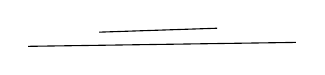
\begin{tikzpicture}\draw (0,0)--(3.4,.05);\draw (.9,.18)--(2.4,.23);\end{tikzpicture}}

% middle, lines 8–14
\[
\left\{\begin{aligned}
t_{\deleted{\unsure{n-}}i}&=\Theta(s'_i)\qquad0\le i\le n+1\\
\langle t_i,\pi\rangle&=-\beta\\
t_i&=\tau_i t_{i+1}\qquad0\le i\le n\\
&\boxed{\begin{aligned}
t_{n+1}=\Theta(s'_{n+1})&=-\sigma a_n^{\prime *}+\gamma\pi=-\sigma a_n^{\prime *}+\gamma a_{n+1}^{\prime *}\\
&=\gamma a_n+(2\gamma-\sigma)a_{n-1}+(\rho'_{n-1,n-1}\gamma-2\sigma)a_{n-2}+\cdots\\
&\quad+(\rho'_{n-1,n-1-j}\gamma\deleted{\unsure{_{n-j}}}-\rho'_{n-2,n-1-j}\sigma)a_{n-j-2}+\cdots\\
&\quad+(\rho'_{n-1,2}\deleted{\unsure{-}}\gamma-\rho'_{n-2,2}\sigma)a_1+\underset{!}{0\cdot a_0}\unsure{-|+}\beta a_{-1}
\end{aligned}}
\end{aligned}\right.
\]

% lower middle, lines 15–16
\[
\begin{aligned}
t_i&=t_{n+1}+\Theta(a'_n+\cdots+a'_i)\\
&=t_{n+1}-\sigma[a_n+\beta_{n-1}a_{n-1}+\beta_{n-1}\beta_{n-2}a_{n-2}+\cdots+(\beta_{n-1}\cdots\beta_i)a_i]
\end{aligned}
\]

% lower middle right, lines 15–16
\[
\Theta(a'_j)=-\sigma(\beta_{n-1}\cdots\beta_j)a_j\qquad0\le j\le n
\]

% lower, lines 17–19
\uline{NB} $t_i=0$ (pour $i$ fixé) sss $\sigma=\gamma=0$ (et \unsure{ceci|celà} implique $\beta=0$)

Si $\beta$ inv. (mais sans que néc. $\sigma$ inv. i.e. $\psi$ iso) alors

On peut définir $-\frac{1}{\beta}t_i\deleted{\unsure{a}}\in\unsure{E|\bar E}\subset X$ \ldots.

% foot, lines 20–22
\[
\begin{aligned}
\varphi(t_{n+1},s_i)&=0\qquad0\le i\le n&\varphi(t_{n+1},s_{n+1})&=\varphi(t_{n+1},a_n)=\beta\sigma\\
\varphi(t_{n+1},a_i)&=0\qquad-1\le i\le n-1\\
f(t_{n+1})&=\tfrac12\langle t_{n+1},\underbrace{\psi(t_{n+1})}_{\beta\sigma s'_{n+1}}\rangle=\frac{\beta\sigma}{2}\gamma=\beta\widetilde{\sigma}\widetilde{\gamma}
\end{aligned}
\]

% foot right, struck draft and replacement
\[
\begin{aligned}
&\deleted{\langle t_{n+1},\psi(a_n)\rangle=(-2\gamma+2\gamma-\sigma)(-\beta)\sigma}\\
&\deleted{=\beta a'_n\,\psi t_{n+1}}\quad\langle a_n,\underbrace{\psi(t_{n+1})}_{\beta\sigma s'_{n+1}}\rangle
\end{aligned}
\]

% foot, left
% archive sheet number: 64

\scanpage{66}
% upright upper left
% letterhead
UNIVERSITE DES SCIENCES\\
ET TECHNIQUES\quad DU LANGUEDOC\\
\texttt{-----}

% upright upper right
% letterhead
\uline{Secrétariat Général}\\
Place\quad Eugène Bataillon\\
\uuline{34060 MONTPELLIER CEDEX}

% upright central heading
\uuline{M A I\qquad 1 9 7 8}

Recueil n° 16

\rule{1em}{.35pt}

% upright right, address label
MR\quad LE PROFESSEUR GROTHENDIECK A.\\
MATHEMATIQUES\hfill 5

% upright central subheading
\uuline{CONSEIL DE L'UNIVERSITE}

\textit{Décisions prises au cours des séances des :}

% upright meeting list, row 1
= 15 Décembre 1977 (116ème séance) ................ Conseil plénier.

% upright meeting list, row 2
= 12 Janvier 1978 (117ème séance) ................. Conseil restreint aux professeurs titulaires.

% upright meeting list, row 3
= 26 Janvier 1978 (118ème séance) ................. Conseil restreint : a) aux membres électeurs au Conseil\\
\hspace*{1em}Scientifique\qquad b) aux membres enseignants du Conseil

% upright meeting list, row 4
= 17 Février 1978 (119ème séance) ................. Conseil restreint aux personnels enseignants, chercheurs, administratifs, techniques, ouvriers et de service.

% upright meeting list, row 5
= 3 Mars 1978 (120ème séance) ..................... Conseil restreint aux enseignants.

% upright meeting list, row 6
= 16 Mars 1978 (121ème séance) .................... Conseil restreint aux professeurs titulaires.

% upright bottom centre
\rule{1em}{.8pt}

% foot, left, in supplied orientation
% archive sheet number: 65

